\pdfbookmark{Общая характеристика работы}{characteristic}             % Закладка pdf
\section*{Общая характеристика работы}
Данная работа посвящена разработке методов анализа изменений в геномах, просходящих на уровне отдельных генов и оперонных структур.

Мы предложили представлять набор геномов в виде графа, в котором хранится информация о всех встречающихся вариантах расположения генов, что позволяет эффективно хранить и визуализировать изменения в сотнях и тысячах геномов. Также мы предложили метод численной оценки уровня изменчивости в отдельных локусах генома и построения профиля локальной изменчивости. 

Отличия в характере локальной изменчивости проиллюстрированы на примере оперонов, значимо чаще встреающихся в изолятах кишечной палочки, полученных от пацентов с болезнью Крона по сравнению с комменсальными штаммами.
\newcommand{\actuality}{\pdfbookmark[1]{Актуальность}{actuality}\underline{\textbf{\actualityTXT}}}
\newcommand{\progress}{\pdfbookmark[1]{Разработанность темы}{progress}\underline{\textbf{\progressTXT}}}
\newcommand{\aim}{\pdfbookmark[1]{Цели}{aim}\underline{{\textbf\aimTXT}}}
\newcommand{\tasks}{\pdfbookmark[1]{Задачи}{tasks}\underline{\textbf{\tasksTXT}}}
\newcommand{\aimtasks}{\pdfbookmark[1]{Цели и задачи}{aimtasks}\aimtasksTXT}
\newcommand{\novelty}{\pdfbookmark[1]{Научная новизна}{novelty}\underline{\textbf{\noveltyTXT}}}
\newcommand{\influence}{\pdfbookmark[1]{Практическая значимость}{influence}\underline{\textbf{\influenceTXT}}}
\newcommand{\methods}{\pdfbookmark[1]{Методология и методы исследования}{methods}\underline{\textbf{\methodsTXT}}}
\newcommand{\defpositions}{\pdfbookmark[1]{Положения, выносимые на защиту}{defpositions}\underline{\textbf{\defpositionsTXT}}}
\newcommand{\reliability}{\pdfbookmark[1]{Достоверность}{reliability}\underline{\textbf{\reliabilityTXT}}}
\newcommand{\probation}{\pdfbookmark[1]{Апробация}{probation}\underline{\textbf{\probationTXT}}}
\newcommand{\contribution}{\pdfbookmark[1]{Личный вклад}{contribution}\underline{\textbf{\contributionTXT}}}
\newcommand{\publications}{\pdfbookmark[1]{Публикации}{publications}\underline{\textbf{\publicationsTXT}}}


{\actuality} В настоящее время накапливается все больше данных о том, что геном прокариот представляет из себя сложно организованную нуклеотидную последовательность. Помимо областей, кодирующих белки или РНК, а также их регуляторных участ, имеется ряд элементов, необходимых для взаимодействия ДНК с молекулярными комплексами, например, теми, которые осуществляют транскрипцию и репликацию. Это делает геном отличным от простого хранилища последовательностей генов, расположенных в случайном порядке, и позволяет говорить об его архитектуре - закономерностях, которые необходимы для успешного функционирования живой клетки.

Новые знания об архитектуре генома могут пролить свет на еще неизвестные подробности основных клеточных процессов и, возможно, облегчить разработку искусственных геномов в области синтетической биологии.


{\progress}
В настоящее время известны некоторые элементы организации геномов. Описан эффект дозировки генов связанный с репликацией: гены, расположенные рядом с сайтом начала репликации, представлены в большем количестве копий в быстро делящихся клетках. Это делает выгодным расположение генов, продукты которых необходимы клетке в больших количествах поблизости от сайта начала репликации. Пространственная укладка ДНК может сближать гены, расположенные в разных областях репликона, что может быть полезно для генов, кодирующих белок-регулятор и его мишени. Экспериментально было установлено, что действие глобальных регуляторов, таких как гистоноподобный белок H-NS, зависят от местоположения генов-мишеней. Склонность к транскрипции (уровень экспрессии генов, не зависящий от их последовательности) значительно меняется в зависимости от положения гена в хромосоме. Взаимодействие РНК-полимераз, возникающее за счет изменения уровня суперскрученности ДНК, может играть роль в регуляции транскрипции соседних генов.

Геномные перестройки и горизонтальный перенос генов могут приводить к изменению оптимального расположения генов и других элементов генома, что может приводить к снижению жизнеспособности организма. Известно, что изменения в геномах преимущественно локализуются в отдельных местах --- "горячих"\ точках. Возможно, эти участки свободны от "архитектурных"\ ограничений, и таким образом более толерантны к изменениям. Возможно, эти участки имеют какие-то признаки, способствующие более высокой частоте происходящих изменений. Нельзя исключать возможности, что "горячие точки"\ возникли в результате генетического дрейфа, их расположение случайно и не обладает функциональным значением. Какие из этих вариантов, и в какой степени, реализуются в действительности, к настоящему моменту, неизвестно: локализация "тихих"\ консервативных участков и "горячих"\ высоко изменчивых локусов не имеет объяснений. Для проведения исследований в данной области необходим инструмент, позволяющий находить и анализировать области генома с повышенной и пониженной изменчивостью. Разработка и применение подобного инструментария и стала основной темой данной работы. 

{\aim} данной работы является разработка програмного конвейера для выявления высокоизменчивых областей прокариотических геномов и применение его для анализа изменчивости в локусах генома \textit{E. coli}, ассоциированных с болезнью Крона.


Для~достижения поставленной цели необходимо было решить следующие {\tasks}:
\begin{enumerate}[beginpenalty=10000] % https://tex.stackexchange.com/a/476052/104425
  \item Разработать, реализовать и проверить эффективность алгоритмов графового представления расположения генов в геномах и оценки уровня изменчивости генома.
  \item Сравнить профили изменчивости геномов для выборок организмов, принадлежащих различным видам и филогруппам (подвидовым структурам) прокариот.
  \item Оценить вклад различных факторов геномной организации в уровень изменчивости генома. 
  \item Разработать алгоритм визуализации подграфов, соответствующих отдельным локусам генома.
  \item Разработать алгоритм выявления, провести поиск и исследовать геномную изменчивость в окрестностях оперонов кишечной палочки, наличие которых ассоциировано с наличием у человека-носителя болезни Крона.  

\end{enumerate}


{\novelty}
\begin{enumerate}[beginpenalty=10000] % https://tex.stackexchange.com/a/476052/104425

Предложенный в нашей работе подход, насколько нам известно, был первым предложенным и реализованным методом для количественной оценки изменчивости генома. 

Насколько нам известно, мы впервые провели сравнение расположения областей повышенной изменчивости у различных видов и внутривидовых структур. Мы обнаружили, что некоторые локусы генома остаются высоко изменчивым для всех представителей вида, в то время, как ряд других локусов являются таковыми лишь у некоторых видов и филогрупп. 


\end{enumerate}

{\influence} \ldots


Изменчивость генома - важный фактор в возникновении штаммов бактерий, обладающих патогенным (или условно-патогенным) фенотипом, в том числе - устойчивостью к антибиотикам. Знание закономерностей подобных трансформаций важно для разработки оптимальных методов контроля над появлением штаммов бактерий, угрожающих жизни и здоровью людей. Возможно, знания о закономерностях изменчивости и консервативности различных областей генома окажется полезными при создании новых последовательностей геномов в области синтетической биологии. 

{\methods} \ldots

{\defpositions}
\begin{enumerate}[beginpenalty=10000] % https://tex.stackexchange.com/a/476052/104425
	\item графовое представления расположения генов в наборе геномов является эффективным средством для визуального анализа изменений геномных изменений и поиска областей генома с повышенной изменчивостью.

	\item Геномы из различных филогрупп и филогенетически близких видов обладают как консервативными (расположенными в схожих местах генома), так и вариативными (присутствующими лишь у некоторых представителей) областями повышенной изменчивости.

 	\item Наибольшее количество областей повышенной изменчивости в рассмотренных геномах находится в областях локализации профагов.

	\item Опероны, значимо чаще встречающиеся в изолятах \textit{E. coli}, изолированных от пациентов с болезнью Крона по сравнению с изолятами полученными от здоровых людей, расположены как в низко-изменчивых областях генома (опероны захвата сорбозы, захвата гимина, утилизации глиоксилата), так и в высокоизменчивых областях (оперон утилизации пропандиола, синтеза и экспорта капсульных полисахаридов).

\end{enumerate}


{\reliability} предложенного метода обосновывается результатами компьютерного моделирования. Результаты находятся в соответствии с результатами, полученными другими авторами.

{\probation}
Основные результаты работы докладывались~на:
перечисление основных конференций, симпозиумов и~т.\:п.

{\contribution} 
1. Предложены подходы графового представления совакупности генов в геномах и оценки геномной вариабельности на основе выбора подграфа.

2. Написан код на языках R, perl и Snakemake для графового представления набора геномов, автоматизации анализов (исправлении ошибок в гомополимерных областях, поиска контаминаций в наборе прочтений, построения ортогрупп, филогенетического анализа).

3. Проведена сборка последовательностей геномов изолятов \textit{E. coli} полученных от пациентов с болезнью Крона и проведено сравнение их с комменсальными штаммами.

4. Проведен анализ расположения областей повышенной изменчивости у различных видов и внутривидовых структурах прокариот.


\ifnumequal{\value{bibliosel}}{0}
{%%% Встроенная реализация с загрузкой файла через движок bibtex8. (При желании, внутри можно использовать обычные ссылки, наподобие `\cite{vakbib1,vakbib2}`).
    {\publications} Основные результаты по теме диссертации изложены
    в~XX~печатных изданиях,
    X из которых изданы в журналах, рекомендованных ВАК,
    X "--- в тезисах докладов.
}%
{%%% Реализация пакетом biblatex через движок biber
    \begin{refsection}[bl-author, bl-registered]
        % Это refsection=1.
        % Процитированные здесь работы:
        %  * подсчитываются, для автоматического составления фразы "Основные результаты ..."
        %  * попадают в авторскую библиографию, при usefootcite==0 и стиле `\insertbiblioauthor` или `\insertbiblioauthorgrouped`
        %  * нумеруются там в зависимости от порядка команд `\printbibliography` в этом разделе.
        %  * при использовании `\insertbiblioauthorgrouped`, порядок команд `\printbibliography` в нём должен быть тем же (см. biblio/biblatex.tex)
        %
        % Невидимый библиографический список для подсчёта количества публикаций:
        \printbibliography[heading=nobibheading, section=1, env=countauthorvak,          keyword=biblioauthorvak]%
        \printbibliography[heading=nobibheading, section=1, env=countauthorwos,          keyword=biblioauthorwos]%
        \printbibliography[heading=nobibheading, section=1, env=countauthorscopus,       keyword=biblioauthorscopus]%
        \printbibliography[heading=nobibheading, section=1, env=countauthorconf,         keyword=biblioauthorconf]%
        \printbibliography[heading=nobibheading, section=1, env=countauthorother,        keyword=biblioauthorother]%
        \printbibliography[heading=nobibheading, section=1, env=countregistered,         keyword=biblioregistered]%
        \printbibliography[heading=nobibheading, section=1, env=countauthorpatent,       keyword=biblioauthorpatent]%
        \printbibliography[heading=nobibheading, section=1, env=countauthorprogram,      keyword=biblioauthorprogram]%
        \printbibliography[heading=nobibheading, section=1, env=countauthor,             keyword=biblioauthor]%
        \printbibliography[heading=nobibheading, section=1, env=countauthorvakscopuswos, filter=vakscopuswos]%
        \printbibliography[heading=nobibheading, section=1, env=countauthorscopuswos,    filter=scopuswos]%
        %
        \nocite{*}%
        %
        {\publications} Основные результаты по теме диссертации изложены в~\arabic{citeauthor}~печатных изданиях,
        \arabic{citeauthorvak} из которых изданы в журналах, рекомендованных ВАК\sloppy%
        \ifnum \value{citeauthorscopuswos}>0%
            , \arabic{citeauthorscopuswos} "--- в~периодических научных журналах, индексируемых Web of~Science и Scopus\sloppy%
        \fi%
        \ifnum \value{citeauthorconf}>0%
            , \arabic{citeauthorconf} "--- в~тезисах докладов.
        \else%
            .
        \fi%
        \ifnum \value{citeregistered}=1%
            \ifnum \value{citeauthorpatent}=1%
                Зарегистрирован \arabic{citeauthorpatent} патент.
            \fi%
            \ifnum \value{citeauthorprogram}=1%
                Зарегистрирована \arabic{citeauthorprogram} программа для ЭВМ.
            \fi%
        \fi%
        \ifnum \value{citeregistered}>1%
            Зарегистрированы\ %
            \ifnum \value{citeauthorpatent}>0%
            \formbytotal{citeauthorpatent}{патент}{}{а}{}\sloppy%
            \ifnum \value{citeauthorprogram}=0 . \else \ и~\fi%
            \fi%
            \ifnum \value{citeauthorprogram}>0%
            \formbytotal{citeauthorprogram}{программ}{а}{ы}{} для ЭВМ.
            \fi%
        \fi%
        % К публикациям, в которых излагаются основные научные результаты диссертации на соискание учёной
        % степени, в рецензируемых изданиях приравниваются патенты на изобретения, патенты (свидетельства) на
        % полезную модель, патенты на промышленный образец, патенты на селекционные достижения, свидетельства
        % на программу для электронных вычислительных машин, базу данных, топологию интегральных микросхем,
        % зарегистрированные в установленном порядке.(в ред. Постановления Правительства РФ от 21.04.2016 N 335)
    \end{refsection}%
    \begin{refsection}[bl-author, bl-registered]
        % Это refsection=2.
        % Процитированные здесь работы:
        %  * попадают в авторскую библиографию, при usefootcite==0 и стиле `\insertbiblioauthorimportant`.
        %  * ни на что не влияют в противном случае
        \nocite{vakbib2}%vak
        \nocite{patbib1}%patent
        \nocite{progbib1}%program
        \nocite{bib1}%other
        \nocite{confbib1}%conf
    \end{refsection}%
        %
        % Всё, что вне этих двух refsection, это refsection=0,
        %  * для диссертации - это нормальные ссылки, попадающие в обычную библиографию
        %  * для автореферата:
        %     * при usefootcite==0, ссылка корректно сработает только для источника из `external.bib`. Для своих работ --- напечатает "[0]" (и даже Warning не вылезет).
        %     * при usefootcite==1, ссылка сработает нормально. В авторской библиографии будут только процитированные в refsection=0 работы.
}

При использовании пакета \verb!biblatex! будут подсчитаны все работы, добавленные
в файл \verb!biblio/author.bib!. Для правильного подсчёта работ в~различных
системах цитирования требуется использовать поля:
\begin{itemize}
        \item \texttt{authorvak} если публикация индексирована ВАК,
        \item \texttt{authorscopus} если публикация индексирована Scopus,
        \item \texttt{authorwos} если публикация индексирована Web of Science,
        \item \texttt{authorconf} для докладов конференций,
        \item \texttt{authorpatent} для патентов,
        \item \texttt{authorprogram} для зарегистрированных программ для ЭВМ,
        \item \texttt{authorother} для других публикаций.
\end{itemize}
Для подсчёта используются счётчики:
\begin{itemize}
        \item \texttt{citeauthorvak} для работ, индексируемых ВАК,
        \item \texttt{citeauthorscopus} для работ, индексируемых Scopus,
        \item \texttt{citeauthorwos} для работ, индексируемых Web of Science,
        \item \texttt{citeauthorvakscopuswos} для работ, индексируемых одной из трёх баз,
        \item \texttt{citeauthorscopuswos} для работ, индексируемых Scopus или Web of~Science,
        \item \texttt{citeauthorconf} для докладов на конференциях,
        \item \texttt{citeauthorother} для остальных работ,
        \item \texttt{citeauthorpatent} для патентов,
        \item \texttt{citeauthorprogram} для зарегистрированных программ для ЭВМ,
        \item \texttt{citeauthor} для суммарного количества работ.
\end{itemize}
% Счётчик \texttt{citeexternal} используется для подсчёта процитированных публикаций;
% \texttt{citeregistered} "--- для подсчёта суммарного количества патентов и программ для ЭВМ.

Для добавления в список публикаций автора работ, которые не были процитированы в
автореферате, требуется их~перечислить с использованием команды \verb!\nocite! в
\verb!Synopsis/content.tex!.
 % Характеристика работы по структуре во введении и в автореферате не отличается (ГОСТ Р 7.0.11, пункты 5.3.1 и 9.2.1), потому её загружаем из одного и того же внешнего файла, предварительно задав форму выделения некоторым параметрам

%Диссертационная работа была выполнена при поддержке грантов \dots

%\underline{\textbf{Объем и структура работы.}} Диссертация состоит из~введения,
%четырех глав, заключения и~приложения. Полный объем диссертации
%\textbf{ХХХ}~страниц текста с~\textbf{ХХ}~рисунками и~5~таблицами. Список
%литературы содержит \textbf{ХХX}~наименование.

\pdfbookmark{Содержание работы}{description}                          % Закладка pdf
\section*{Результаты}

\subsection*{Графовое представление геномов}

Нами был предложен и реализован метод представления набора геномов в виде графа. Гены, относящиеся к одной ортогруппе, представляются в виде узла графа, а ребра отражают взаимное расположение генов в геномах. Ребро проводится между двумя узлами в том случае, если соответствующие гены расположены по соседтсву хотя бы в одном геноме; чем в большем количестве геномов наблюдается такое расположение генов, тем выше вес ребра (Рис 1 А).

Преложенная схема требует уточнения в случае, когда несколько генов из одной геномной последовательности принадлежат к одной ортогруппе (мы будем называть такие гены паралогами). Мы предложили два подхода представления паралогичных генов в графе. В первом случае мы игнорируем паралогичные гены и не добавляем их в граф. Во втором --- мы проводим процедуру "ортологизации"\ паралогичных генов: гены из ортогруппы добавляем в граф с некоторым суффиксом, при этом гены имеющие одинаковый контекст добавляются с одним и темже суффиксом. В нашей програмной реализации пользователь может выбирать применяемый подход. 

В случае геномов прокариот, визуализация полного графа будет не наглядна и сложна для проведения зрительного анализа. Практический интерес представляет анализ подграфов, соответствующих определенному региону генома. Мы разработали процедуру построения подграфа --- подмножества узлов и ребер, которые отражают набор генов выбранного участка одного референсного генома и набора геномов сравнения. 

Первым шагом алгоритма является построение \textit{референсной цепочки узлов} --- узлов графа, которые соответствуют генам референсного генома расположенным в выбранном регионе. Далее, в подграф включаются все пути, которые начинаются и заканчиваются на референсной цепочке. Мы предусмотрели несколько фильтров, позволяющих снизить количество отображаемымых узлов и ребер. Фильтр минимального веса ребра позволяет отсечь ребра, которые представляют редкие сочетания генов (встречающиеся в небольшом количестве геномов). Фильтр длинных путей заменяет слишком протяженные цепочки узлов (могут появиться в результате геномных перестроек) на короткие фрагменты ("хвосты"\ ) некоторой заданной длины (Рис 3). 

Визуализация подграфов обладает практической ценностью, поскольку позволяет создавать наглядную визуализацию возможных сочетаний генов в определенной области генома. Подобный тип визуализации можно использовать для определения того, представлен ли некоторый оперон в одном и том же генном контексте, или в разных. Под генным контекстом мы понимаем гены, расположеные непосресдвенно перед и после оперона. Мы говорим об одинаковом контексте в случае, если гены перед опероном относятся к одной ортогруппе, и гены после оперона относятся к некоторой другой ортогруппе; в графовом представлении, при этом, мы будем наблюдать, что цепочка узлов, соответствующая генам оперона, будет соединена с одним узлом с одной стороны и с другим узлом --- с другой. Иллюстрация расположения оперонов утилизации гемина и пропандиола в 325 геномных последовательностях различных изолятов кишечной палочки приведенеа на (Рис 3). Данные опероны статистически чаще встречаются в изолятах кишечных палочек, полученных от пациентов с болезнью Крона (об этом речь будет идти ниже).

Обращает на себя внимание значительная разница в уровне сложности подграфов показанных на Рис 4. Эта сложность (количество узлов и ребер) отражает разное количество изменений генного состава, зафиксированных в ходе эволюции в данных областях генома. Мы предложили использовать графовое представление для оценки локальной изменчивости генома. 

\subsection*{Оценка изменчивости геномов при помощи графового представления}
В качестве меры локальной изменчивости геномов мы предложили использовать подсчет количества путей в соответствующем подграфе. В случае, если в некотором регионе не происходит изменений генного состава, то подграф представляет из себя простую структуру с одним возможным путем (способом обхода узлов). В случае, если в данной области происходят изменения, то в подграфе появляются новые пути. Чем больше различных вариантов сочетания генов наблюдаются в геномных последовательностях, тем больше путей в соответствующем подграфе. 

Оценка локальной вариабельности производится для одного гена референсного генома с учетом окна (смежных генов), размер которого можно задавать при запуске алгоритма. Алгоритм рассчета состаит в следающем. Вначале строится референсная цепочка узлов, после чего происходит подсчет путей, которые огибают узел(начинаются по одну сторону, а заканчиваются -- по другую) (Рис 5). Подсчет числа путей в графе --- сложная вычислительная задача, относящаяся к классу NP-полных (время решения экспоненциально зависит от размера графа). Поэтому мы выбрали вероятностный подход к подсчету числа путей. Мы задаем максимальное значение итераций и каждую итерацию ищем путь, начиная с первого узла референсной цепочки и затем выбирая следующие вершины случайным образом, пока путь не вернется в референсную цепочку, либо пока не будет достигнуто максмальное количество переходов. Количество найденных различающихся путей мы считаем мерой локальной изменчивости. Реализация метода доступна в пакете gene-graph-lib для языка Python.

\subsection*{Верификация и анализ применимости метода оценки локальной изменчивости}
Для верификации предложенного алгоритма и его програмной реализации мы провели компьютерное моделирование эволюции геномов. Для каждого локуса моделируемого генома мы задавали опреленный уровень вариабельности, вероятностным образом измененяли генный состава и потом оценивали вариабельность при помощи предложенного нами подхода. Изменения генного состава происходили за счет вставки, удаления либо перемещения генов а также инверсий фрагментов генома. Вероятность инверсий была в 100 рез меньше вероятностей остальных событий, а размер области для инверсии выбирался случайно из экспоненциального распределения. Локализация событий изменений генного состава выбиралась случайно в соответствии с распределенией уровня вариабельности. Значения локальной вариабельности задавались в соответствии с одним из типов профилей: пилообразным, прямоугольным либо синусоидальным (Рис 6). На Рис6 показано сравнение изначально заданных профилей вариабельности и значений, полученных предложенным нами методом оценки локальной вариабельности. Уровень корреляции был выше ...


\subsection*{Анализ расположения областей повышенной изменчивости в геномных последовательностях кишечной палочки}
Для проведения данного анализа мы собрали коллекцию из 327 геномов бактерии \textit{E. coli} доступных в базе данных RefSeq, построили группы гомологии при помощи программы Orthofinder и применили разработанной нами метод оценки уровня геномной вариабельности, в качестве референсного генома был выбран геном штамма LF82, изолированного из пациента с болезнью Крона. На рисунке X показан профиль изменчивости и области расположения профагов, островов патогенности, генов рекомбиназ (для выявления следов мобильных элементов генома), жизненно необходимых генов (мутации в которых являются летальными) и генов транспортных и рибосомальная РНК.

\begin{figure}[!ht] 
    \center
      \includegraphics[width=\textwidth]{Dissertation/images/complexity/figure5plus.png}
    \caption{Профиль вариабельности генома \textit{Escherichia coli LF82}. Цветом обозначены острова патогенности, профаги,  гены, ассоциированные с мобильными элементами генома, жизненно-необходимые гены, гены транспортных и рибосомных РНК. Области повышенной изменчивости содержат меньше жизненно-необходимых генов. Профаги и острова патогенности обладают повышенным уровнем изменчивости по сравнению с остальной частью генома.}
    \label{img:complexity_lf82} 
  \end{figure}

Можно заметить, что участки генома в которых расположены жизненно необходимые гены, как правило, мало изменчивы а к высокоизминчивым областям генома относятся профаги и острова патогенности. При этом, наблюдаются также высоко изменчивые области генома, в которых отсутствуют признаки мобильных элементов; причины их высокой изменчивости остаются неизвестными. 

Гены транспортных РНК не проявлят явной ассоциации с профилем изменчивости. Гены рибосомальной РНК находятся преимущественно в мало изменчивых областях генома. 

Время существования вида \textit{Escherichia coli} оценивается в несколко десятков миллионов лет; возникает вопрос об устойчивости расположения горячих областей генома с течением времени. Для анализа этого вопроса мы провели сравнение профилей изменчивости подвидовых структур.  Для кишечной палочки существует устоявшаяся классификация клад филогенетического дерева,  называемых филогруппами.  Для создания набора геномов мы выбрали по одному представителю из наиболее крупных филогрупп (A, B1, B2, E) и подобрали для каждого из них  по сто ближайший геномов из базы NCBI RefSeq. Филогенетическое дерево подобранных таким образом геномов показано на рисунке~\ref{img:phylogroups}. 

\begin{figure}[!ht] 
    \center
      \includegraphics[width=0.65\textwidth]{Dissertation/images/complexity/coli_phylogroups.png}
    \caption{Филогенетическое дерево выборки геномов \textit{E. coli}, состоящей из представителей пяти крупных филогрупп: A, B1, B2, D, E (обозначены зеленым, черным, оранжевым, синим, красным цветом соответственно).}
    \label{img:phylogroups} 
  \end{figure} 

Затем мы рассчитали профили изменчивости для каждой филогруппы в отдельности и сравнили их между собой. Результат сравнения показан на рисунке~\ref{img:phylogroups_complex}, серым цветом обозначены блоки синтении, оранжевым -- области нахождения профагов.    

\begin{figure}[!ht] 
    \center
      \includegraphics[width=\textwidth]{Dissertation/images/complexity/coli_phylogroups_complexity_3.png}
    \caption{Сравнение профилей вариабельности представителей пяти филогрупп \textit{E. coli LF82}. Оранжевым цветом выделены области, определенные как профаговые. Блоками серого цвета показаны области синтении.}
    \label{img:phylogroups_complex} 
  \end{figure}
  

Сравнение показывает, что ряд областей генома с повышенной изменчивостью присутствуют во всех или в большинстве филогрупп, что по-видимому свидетельствует об их длительном существовании на протяжении значительной части времени жизни вида. Часть из этих областей соответствуют местам расположение профагов и их устойчивость можно объяснить сайт специфичным характером встраивания данных элементов. Одна из устойчивых горячих точек не имеет выявленных признаков мобильных элементов генома (рисунок~\ref{img:phylogroups_complex} В). Также можно выделить области генома, обладающие повышенной изменчивостью лишь у одной или нескольких филогрупп (рисунок~\ref{img:phylogroups_complex} Б, Г).

Значительная часть горячих областей геномов являются местами встройки фагов, что особенно заметно на примере филогруппы E, для которой была описана вирусная экспансия, значительно удлинившая их геномную последовательность (на рисунке длины геномов приведены к одинаковой ширине, но о размере генома можно судить по координатным осям ниже пролфилей изменчивости).

Заметно также существование и "холодных"\ областей генома с низкой вариабельностью во всех филогруппах. Длина этих маловариабельных участков может значительно превышать характерные длины оперонов, и достигать величин порядка миллиона пар оснований (например, область в окрестности 4 млн. п.н. на рисунке~\ref{img:phylogroups_complex} А.

\subsection*{Анализ изменчивости геномов у двух видов рода \textit{Pseudomonas}}

Мы повторили анализ расположения областей повышенной изменчивости у двух видов псевдоманад: \textit{Pseudomonas aeruginosa}, \textit{Pseudomonas fluorescens}. Данные виды были выбраны как представители бактерий, для которых характерна высокая частота рекомбинационных событий. \textit{Pseudomonas} - род грамотрицательных бактерий, отдельные виды которого значительно различаются по метаболическому потенциалу и занимаемым экологическим нишам. \textit{P. fluorescens} обитают преимущественно в почве и являются естественно компетентными. \textit{P. aeruginosa} - оппортунистические патогены человека, компетентность которых наблюдалась лишь в условиях жизни в биопленке. Для каждого рассмотренного вида мы использовали последоватеьлности геномов доступные в базе RefSeq, построили для них филогенетическое дерево, выбирали наиболее крупные клада дерева и провели анализ изменчивости в каждой кладе независимо. Результаты сравнения показаны на рисунке~\ref{img:pseudo_complexity}. 

\begin{figure}[!ht] 
  \center
    \includegraphics[width=\textwidth]{Dissertation/images/complexity/pseudo_complexity.png}
  \caption{Сравнение профилей вариабельности двух клад вида  А) \textit{P. aeruginosa} и Б) \textit{P. fluorescens}. Оранжевым цветом выделены области, определенные как профаговые.}
  \label{img:pseudo_complexity} 
\end{figure}

В случае \textit{P. aeruginosa} наблюдается значительное сходство профилей изменчивости геномов из двух клад (рисунок~\ref{img:pseudo_complexity} А). В случае {P. fluorescens} подобное сходство выражено слабо и заметно только в небольшом фрагменте ближе к концу хромосомы, после 6 млн. пар оснований, а сами профили вариабельности обладают меньшим количеством выраженных горячих точек (рисунок~\ref{img:pseudo_complexity} Б). Вероятная причина наблюдаемой разницы - высокая частота крупных хромосомных перестроек у \textit{P. fluorescens}. 

Частые хромосомные перестройки делают анализ локальной изменчивости мало информативным, ведь для применимости метода необходимо, во-первых, наличие локальных участков повышенной изменчивости, и во-вторых, чтобы глобальные перестройки хромосомы происходили сравнительно редко относительно локальных изменений (вставки, делеции и транслокации отдельных генов).

\subsection*{Сравнение профилей вариабельности между близкородственными видами}

Предложенный нами подход также применим для сравнения изменчивости у представителей близкородственных видов. Мы провели анализ изменчивости у 143 видов бактерий и архей. Интерактивная визуализация полученных профилей изменчивости доступна на веб-сервере \url{gcb.rcpcm.org}, о котором будет рассказано ниже. Мы проанализировали геномы видов, для которых было доступно не менее 50 полногеномных последовательности.

Для сравнения профилей изменчивости между собой мы расположили их в соответствии с филогенетическим деревом, и нашли участки синтении между парами геномов, расположенными на дереве по соседству. Фрагмент итоговой визуализации показан на рисунке~\ref{img:tree_fragment}, полная визуализация доступна по адресу \url{https://github.com/paraslonic/GCB_revision/blob/master/figures/S3_Fig.pdf}.

\begin{figure}[!ht] 
  \center
    \includegraphics[width=\textwidth]{Dissertation/images/complexity/tree_fragment.png}
  \caption{Фрагмент визуализации профилей изменчивости геномов различных видов. Профили расположены в соответствии с филогенетическим деревом видов, блоки синтении показаны для смежных по дереву видов.   }
  \label{img:tree_fragment} 
\end{figure}

В большинстве случаев, когда между видами наблюдается сохранности геномной структуры (малое количество геномных перестроек), профили изменчивости похожи (области повышенной изменчивости находятся в схожем окружении). 

В качестве примера на рисунке~\ref{img:species_complex_bacillus} А показано сравнение профилей изменчивости четырех видов рода \textit{Bacillus}, филогенетическое дерево для рассмотренных видов показано на рисунке~\ref{img:species_complex_bacillus} В. В геномных последовательностях \textit{B. amyloliquefaciens} и \textit{B. velezensis} заметна крупная инверсия (рис.~\ref{img:species_complex_bacillus} А, выделена рамкой), при этом, области высокой изменчивости сохраняют свое расположение (рис~\ref{img:species_complex_bacillus} Б, пики изменчивости обозначены римскими цифрами). 

\begin{figure}[!ht] 
  \center
    \includegraphics[width=\textwidth]{Dissertation/images/complexity/bacillus_compare_v3.png}
  \caption{Сравнение профилей вариабельности четырех различных видов рода \textit{Bacillus}. А) Профили изменчивости и блоки синтении, оранжевым цветом выделены области, определенные как профаговые, рамка из штрихованных линий показывает фрагмент, представленный на Б). В) Филогенетическое дерево рассматриваемых видов.}
  \label{img:species_complex_bacillus} 
\end{figure}

\subsection*{Связь между уровнем изменчивости и характеристиками генома}\label{chaptComplexWithSMTH}

Профили изменчивости для геномов из различных филогрупп и близкородственных видов показали значительную степень сходства: наблюдается множество "горячих"\ точек изменчивости со стабильным положением в хромосоме. Открытым остается вопрос о причинах этого постоянства, факторах определяющих увеличение либо снижение уровня докальной вариабельности. В качестве первых шагов по выявлению того, что определяет уровень изменчивости мы провели сравнения между профилем изменчивости и расположением Chi\-сайтов, а также частотой межхромосомных контактов. 

\subsubsection*{Связь геномной изменчивости с распределением Chi сайтов.}
Горизонтальный перенос генов требует захвата чужеродной ДНК и эффективной рекомбинации с хозяйсткой ДНК. Ранее, в работе группы Эдуардо Роша, было высказано предположение о значительной роли гомологичной рекомбинации в осуществлении горизонтального переноса генов, приводящего к возникновению областей повышенной изменчивости. Это предположение основано на наблюдении, что в консервативных областях генома, расположенных в непосредственной близости от высокоизменчивых областей, часто встречаются следы рекомбинационных событий. У бактерии \textit{E. coli} описаны Chi сайты, играющие важную роль в инициации процесса гомологичной рекомбинации. Мы предположили, что встречаемость данных сайтов может быть ассоциированна с уровнем изменчивости.

На рисунке~\ref{img:chi_lf82} А показан уровень локальной вариабельности и локализация Chi-сайтов для хромосомы штамма \textit{E. coli LF82}. Из приведенного рисунка видно неравномерное распределение Chi сайтов по реплихорам хромосомы и их сниженная представленность в местах локализации профагов/островов патогенности, а также в иных областях с высокой вариабельностью. На рисунке~\ref{img:chi_lf82} б) показано сравнение уровня вариабельности и расстояний до ближайшего Chi сайта (на соответствующей цепи, лидирующей для правой реплихоры, и отстающей - для левой). Корреляция между уровнем вариабельности и расстоянием до ближайшего Chi-сайта значима (p-value < 1e-16), значение коэффициента корреляции составляет 0.25.

\begin{figure}[!ht] 
  \center
    \subcaptionbox{}{\includegraphics [width=1\textwidth] {Dissertation/images/complexity_with_smth/lf82_chi_sites.png}}
    
    \subcaptionbox{}{\includegraphics [width=1\textwidth] {Dissertation/images/complexity_with_smth/chidist_complexity.png}}
    
    \caption{Уровень вариабельности и локализация Chi-сайтов на двух цепях хромосомы \textit{E. coli LF82}. А) Синие вертикальные линии показывают расположение Chi-сайтов на двух цепях хромосомы. Вертикальные пунктирные линии показывают границы реплихор (места начала и конца репликации). Желтым и красным цветом обозначены области расположения профагов и островов патогенности соответственно. Б) Черной линией показан уровень вариабельности, синей - расстояние до ближайшего Chi сайта (в масштабе тысяч пар оснований).}
    \label{img:chi_lf82}
\end{figure}

Таким образом, мы наблюдаем ассоциацию между высоким уровнем геномной изменчивости и низкой частотой встречаемости Chi сайтов. 

\subsection{Связь геномной изменчивости с плотностью хромосомных контактов}

Одним из экспериментальных методов определения пространственной укладки хромосомы является метод Hi-C, основанный на лигировании фрагментов ДНК расположенных в непосредственной близости друг от друга, с последующим их секвенированием и картированием на линейную геномную последовательность. Результатом работы данного метода является матрица частот межхромосомоных контактов.

На рисунке~\ref{img:hic_matrixes} показано сопоставление профилей вариабельности с матрицами частот межхромосомных контактов для бактерий \textit{E. coli} и \textit{B. subtilis}. Очевидной связи между профилем сложности и частотой хромосомных контактов, с нашей точки зрения, не наблюдается.

\begin{figure}[!ht] 
  \center
    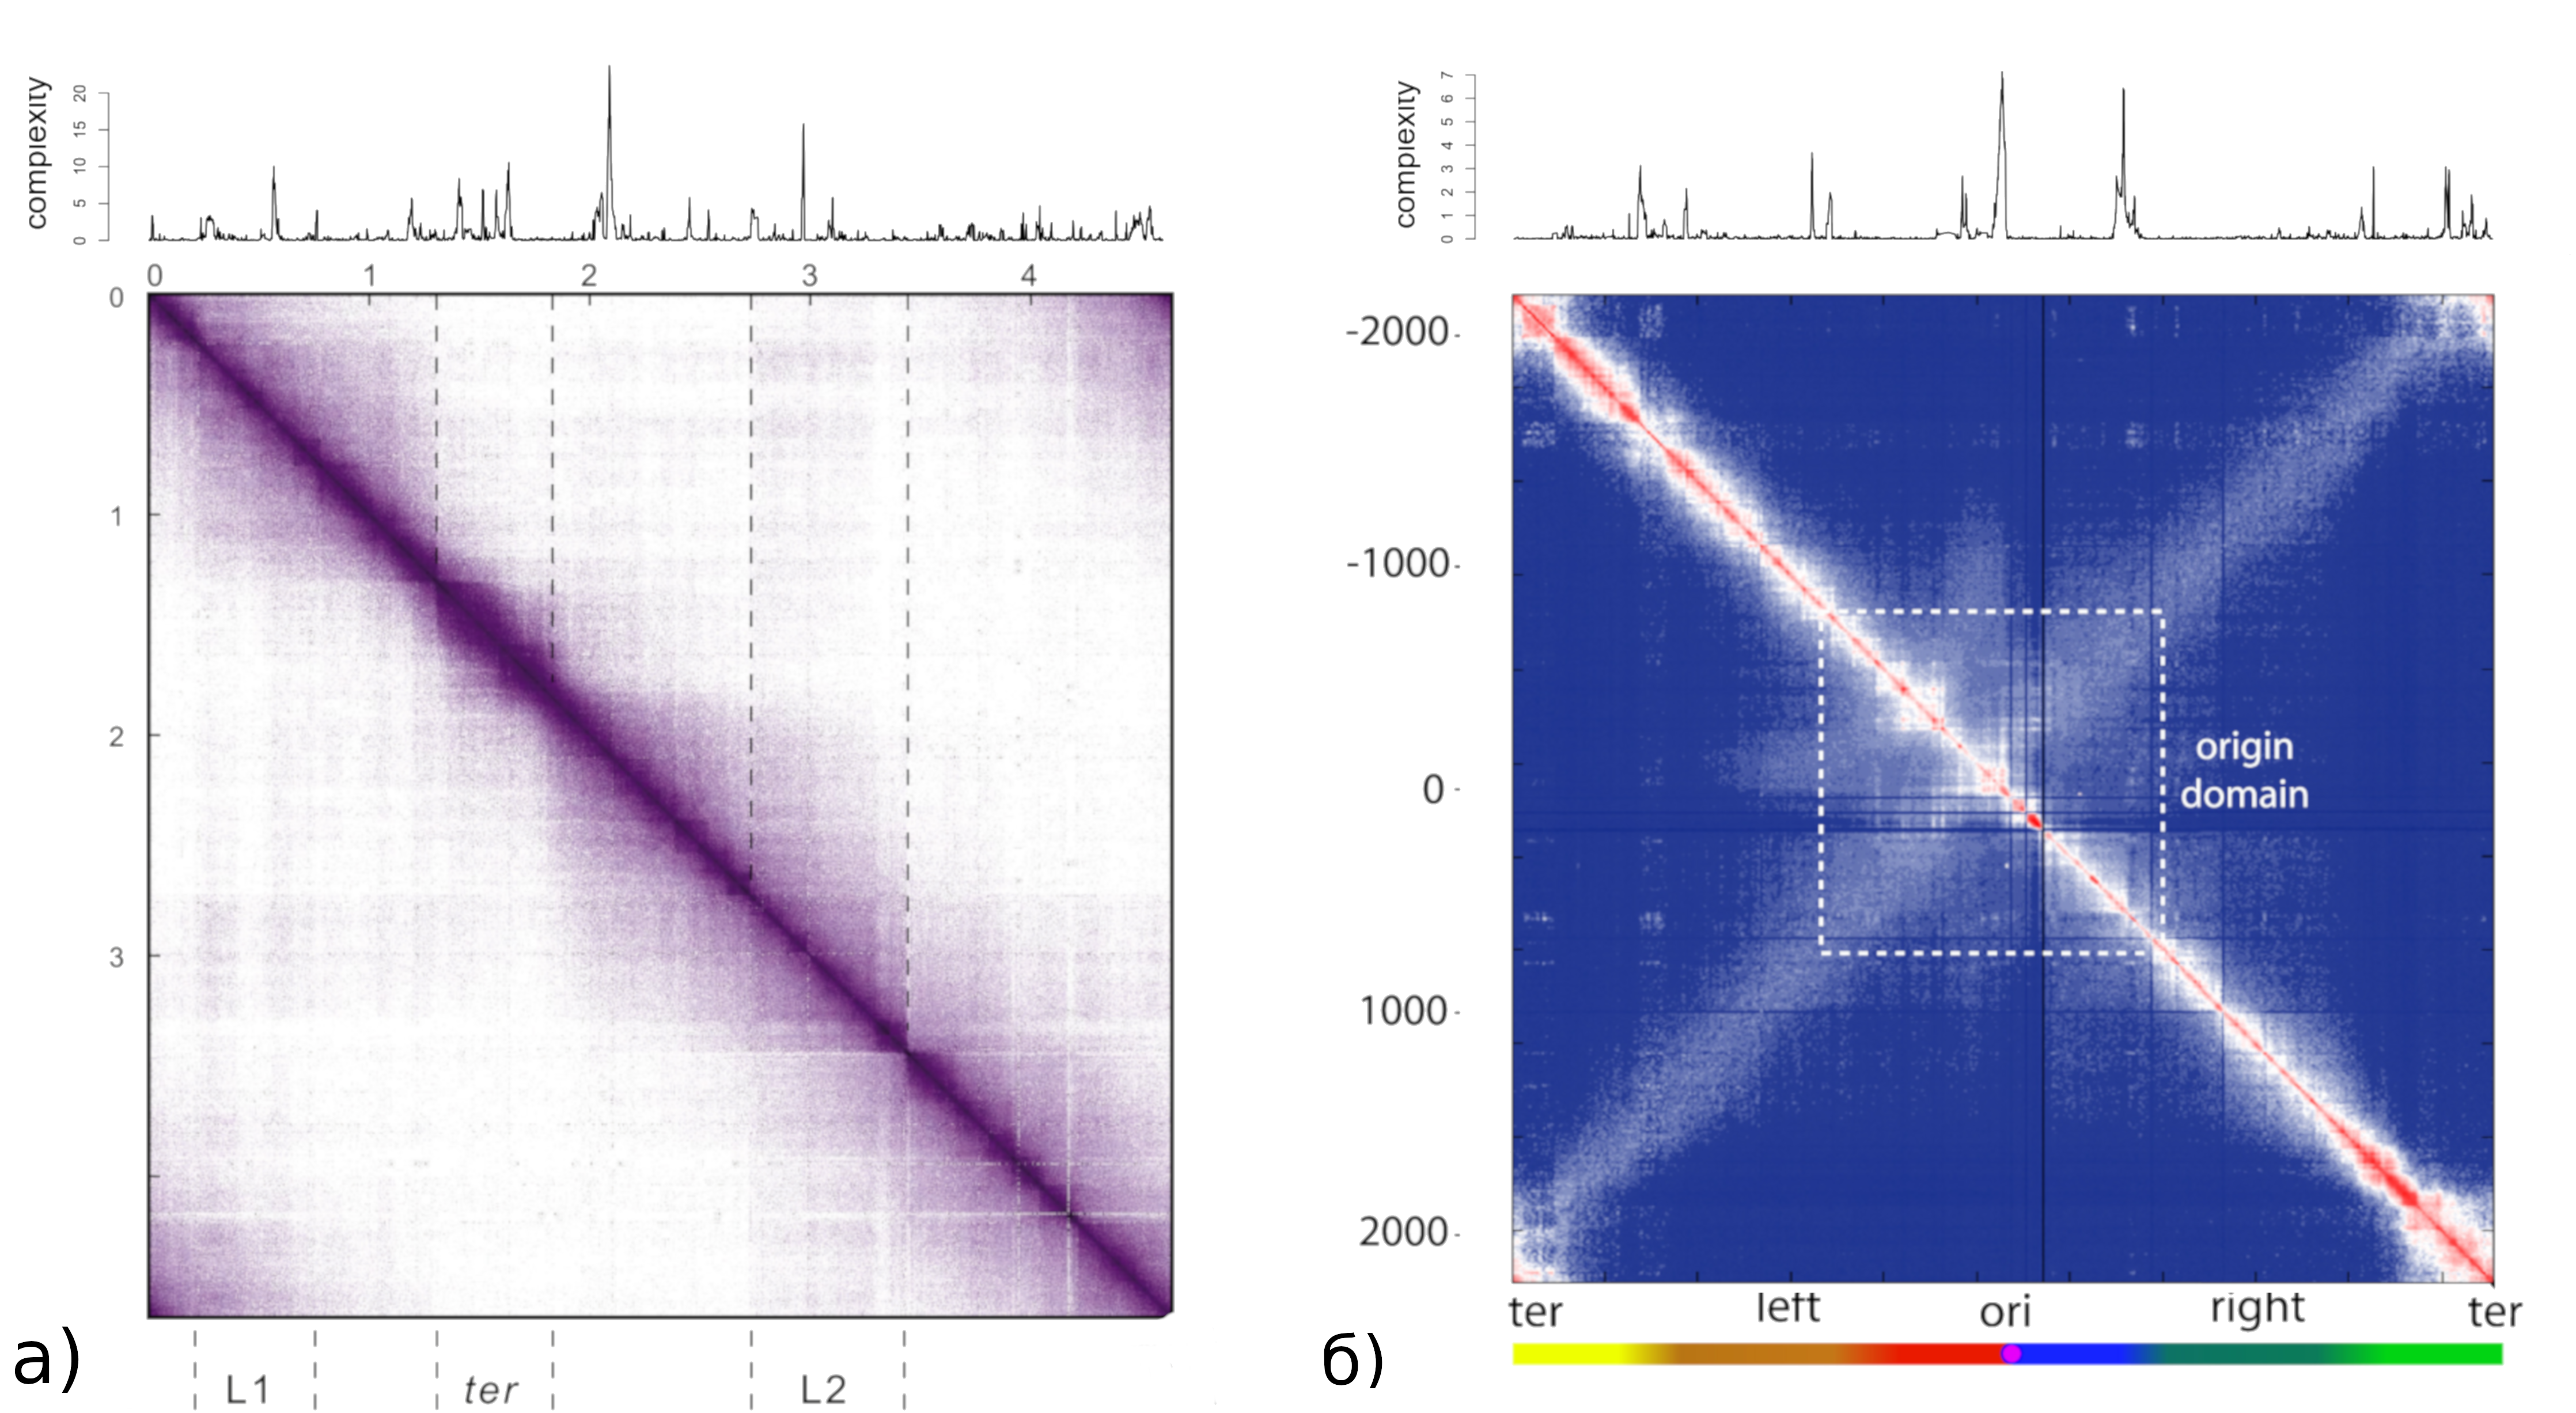
\includegraphics [width=0.9\textwidth] {Dissertation/images/complex_hic/hic_matrixes.png}
    \caption{Сравнение профилей сложности с нормированными матрицами хромосомных контактов для \textit{E. coli} и \textit{B. subtilis}}
    \label{img:hic_matrixes}
\end{figure}

В тоже время, признаки существования подобной связи имеются, при сравнении профиля сложности с шкалограммой, построенной на основе матрицы контактов. Шкаллограмма отражает размер окна в котором необходимо произвести суммирование частот контактов, чтобы достичь определенного перцентильного значения (рисунок~\ref{img:scalogram_complexity_coli}). При помощи метода линейной регрессии нами была выявлена статистически значимая зависимость между уровнем изменчивости генома и локальной суммой межхромосомных контактов в окне определенного размера (размер выбирался так, чтобы лучшим образом соответствовать окну используемому при расчете уровня изменчивости). 
 
\begin{figure}[!ht] 
  \center
    \includegraphics [width=0.9\textwidth] {Dissertation/images/complex_hic/hic_scalogram_complexity_coli.png}
    \caption{Сравнение профиля сложности с шкаллограммой хромосомных контактов из публикации \cite{lioy2018multiscale}.}
    \label{img:scalogram_complexity_coli}
\end{figure}

Как и в случае с распределением Chi сайтов, ассоциация между уровнем изменчивости и плотностью межхромосомных контактов является статистически значимой, но довольно слабой (значение $R^2$ для \textit{E. coli} составляет 0.04, а для \textit{B. subtilis} $R^2 = 0.06$).

\subsection*{Разработка и применение графового подхода для анализа локальной вариабельности геномов}

Множество сочетаний генов, которые наблюдаются в наборе геномов, можно представить в виде графа и использовать его для визуализации сравнений геномных последовательностей. Преимуществом данного подхода является компактность визуализации, так что становится возможным сравнение генных контекстов в сотнях геномных последовательностях. Компактность достигается за счет того, что консервативное сочетание генов (встречающиеся в большом количестве геномов) представлено на визуализации при помощи одного ребра, вне зависимости от количества геномов. Новые узлы и ребра добавляются в граф только в случае, когда ранее подобные сочетания не наблюдались. 

Визуализация полного графа для набора геномов возможна в случае небольших вирусных геномов; в случае бактериальных геномов имеет смысл проводить визуализацию и анализ подграфа --- части полного графа, соответствующей некоторому региону интереса (например, оперону).

Для построения подграфа мы реализовали следующий алгоритм. Вначале выбирается референсный геном и указывается начало и конец анализируемой области. Затем, строится граф, содержащий цепочку узлов референсного генома и к нему добавляются узлы, представленные в других геномах и связанные с референсной цепочкой. Добавление узлов происходит пока путь снова не вернется в референсную цепочку, либо пока не будет достигнуто ограничение на длину (задается параметром \textit{tails}).

Даже при рассмотрении небольшого участка генома, соответствующий ему подграф может содержать длинные пути, которые затрудняют визуализацию. Подобные пути могут появиться например, из-за крупных хромосомных перестроек. Для того, чтобы эти длинные пути не затрудняли визуализацию и последующий анализ, в алгоритме предусмотрен фильтр, который заменяет длинный путь его начальным и концевым фрагментом ("усами"). Максимальная длина пути, который будет показан полностью, задается параметром \textit{max\_depth}, размер фрагментов, которые сохраняются вместо длинного пути (длина "усов") задается параметром \textit{tails} (рисунок~\ref{img:tails_schema}). Пути, которые начинаются либо заканчиваются, но не начинаются и заканчиваются, в рассматриваемой области ("уходящие" за пределы рассматриваемой области) также сокращаются до фрагментов длиной \textit{tails}. Еще один фильтр позволяет не включать в подграф ребра с маленьким весом, то есть те, которые встречаются в малом количестве геномов. За это отвечает параметр \textit{minimal\_edge\_weight}. Применение фильтров особенно важно при анализе "горячих" точек изменчивости.

\begin{figure}[!ht] 
  \center
  \includegraphics[width=0.8\textwidth]{Dissertation/images/subgraphs/tails_schema_v2.png}
  \caption{Схематическая иллюстрация работы фильтра длинных путей. }
  \label{img:tails_schema} 
\end{figure}

\subsection*{Примеры применения графового подхода для визуализации сравнения геномов}

В работе \cite{rakitina2017genome}, нами были установлены опероны, которые статистически значимо чаще встречались у изолятов \textit{E. coli} полученных от пациентов болезнью Крона (воспалительное заболевание кишечника), по отношению к изолятам от здоровых людей. Носительство данных оперонов, вероятно, выгодно при нахождении бактерий в условиях воспалительной реакции со стороны организма хозяина, а может и провоцирует воспаление. Метод для поиска оперонов, различающих группы бактерий, будет описан ниже.

Рассмотрим, как выглядят подграфы, соответствующие некоторым из выявленых оперонов. На этих примерах будут проиллюстрированы основные моменты анализа графового представления фрагментов генома. 

\textbf{Опероны утилизации гемина и пропандиола}

На рисунках~\ref{img:sub_hem} и ~\ref{img:sub_pdu} показаны графы, построенные в окрестностях оперонов захвата гемина (hemin uptake, hmu) и утилизации пропандиола (propanediol utilization operon, pdu), соответственно. В качестве референсного генома нами был взят геном \textit{Escherichia coli LF82}, в анализ были включены 327 финишированных геномов доступных в базе RefSeq. Для построения данных графов мы использовали следующие параметры: \textit{tails} = 1, \textit{max\_depth} = 30, \textit{minimal\_edge\_weight} = 5. 

Рассмотрим для начала более простой случай оперона захвата гемина. Как видно из графа, представленного на рисунке~\ref{img:sub_hem}, данный оперон расположен в консервативном генном контексте. Дуговое ребро выходящее оперон сверху говорит о том, что в некотором наборе геномов данный оперон отсутствует и других последовательностей генов в этом локусе не наблюдается. 

\begin{figure}[!ht] 
  \center
  \includegraphics[width=0.8\textwidth]{Dissertation/images/subgraphs/hemin.png}
  \caption{Граф представляющий окрестность оперона утилизации гемина (hemin uptake, hmu).}
  \label{img:sub_hem} 
\end{figure}

Для оперона утилизации пропандиола также наблюдается консервативность его рассположения. Ребро обходящее оперон (дуга ниже оперона) говорит о том, что в ряде штаммов в данном контексте нет иных вариантов последовательностей генов. Наблюдается некоторая вариабельность внутри оперона, соответствующая нескольким вариантам данного оперона \cite{rakitina2017genome}. Помимо pdu оперона, в том же контексте, у ряда штаммов наблюдается альтернативный набор последовательностей генов. В этот альтернативный набор входят гены транспорта железа (FepC, FcuA, HmuU), гены мобильных элементов (retroviral integrase core domain, transposase DDE Tnp ISL3) и множество гипотетических генов с неизвестной функцией. Примечательна вариабельность этого альтернативного набора генов. Вероятно, данный участок генома часто служит местом рекомбинационных событий, приводящих к изменению набора генов, причем эти изменения не имеют строгого начала и конца (т.е. не сайт специфичны), но часто накладываются друг на друга. 

\begin{figure}[!ht] 
  \center
    \includegraphics[width=0.8\textwidth]{Dissertation/images/subgraphs/pdutail1minw2_v2.pdf}
  \caption{Граф представляющий окрестность оперона утилизации пропандиола (propanediol utilization operon, pdu). }
  \label{img:sub_pdu} 
\end{figure}

\textbf{Кластер генов синтеза бактериальной капсулы}

Перейдем к описанию графа, представляющего окружение оперона синтеза капсулы, также чаще встречающегося у изолятов из пациентов с болезнью Крона. На рисунке~\ref{img:capsule_sub_small} показано ближайшее окружение данного оперона, сам оперон обведен рамкой серого цвета. 

\begin{figure}[!ht] 
  \center
    \includegraphics[width=\textwidth]{Dissertation/images/subgraphs/capsular_subgraph.png}
  \caption{Граф представляющий окрестность кластера генов синтеза бактериальной капсулы. }
  \label{img:capsule_sub_small} 
\end{figure}

Видно, что оперон состоит из консервативных фрагментов, фланкирующих вариабельный участок. Вариабельная часть оперона соответствует генам, отвечающим за синтез серотип-специфичного набора полимеров капсулы; гены консервативной части кодируют белки, участвующие в транспорте синтезированных веществ через клеточную стенку.

Фрагменты единичной длины, расположенные на рисунке~\ref{img:capsule_sub_small} слева от оперона, говорят о том, что есть много путей, которые не попадают в построенный подграф поскольку либо слишком длинные, либо заканчиваются вне отображаемой области и поэтому были сокращены до коротких фрагментов (параметр \textit{tails} при анализе был равен 1). Если расширить рассматриваемую окрестность оперона, то многие из этих путей станут видны, поскольку теперь они будут начинаться и заканчиваться в рассматриваемой области (рисунок~\ref{img:capsule_sub_large}). Вид данного графа говорит о значительной вариабельности участка генома, содержащего гены синтеза капсулы.

\begin{figure}[!ht] 
  \center
    \includegraphics[width=\textwidth]{Dissertation/images/subgraphs/capsular_subgraph.pdf}
  \caption{Граф для расширенной окрестности генов синтеза бактериальной капсулы. }
  \label{img:capsule_sub_large} 
\end{figure}

Вариабельность состава капсулы адаптивна, она помогает бактериям избегать распознавание иммунной системой организма-хозяина и бактериофагами. Можно выдвинуть гипотезу, что данный участок генома обладает некоторыми (еще не установленными) свойствами, которые обеспечивают его значительную вариабельность, что способствует вариабельности состава генов капсулы. С другой стороны, такое расположение оперона может быть обьяснено его горизонтальным переносом (который более вероятен в областях с повышенной изменчиовостью).



\subsection*{Алгоритмизация подхода выявления оперонов, наличие которых ассоциировано с определенным признаком. } \label{chaptOperons}

Предположим, что у нас есть некоторый признак, по которому мы можем разбить набор геномов на группы, и наша задача --- установить, какие гены значимо чаще (либо реже) встречаются в одной из групп. Простым и распространенным методом анализа, в подобном случае, является вычисление статистики и оценка значимости по каждому отдельному гену. После проведения этих тестов необходимо применить поправку на множественное сравнение, так как иначе следует ожидать множество ложно положительных результатов. В случае, если работа ведется на данных о полной последовательности генома, имеется большое количество анализируемых генов (порядка $10^3 - 10^4$), а размеры групп, как правило, незначительны (порядка $10^1 - 10^2$), что приводит к тому, что после поправки на множественное сравнение, ни один из анализируемых генов не проходит даже низкие пороги на значимость. В качестве одного из способов преодоления описанной выше проблемы мы предложили использовать информацию об организации генов в опероны для поиска значимых ассоциаций \cite{rakitina2017genome}. Рассматривая оперон как структурную единицу, мы значительно сокращаем количество анализируемых признаков.

\textbf{Алгоритм поиска генетических ассоциаций}
На входе необходимо иметь два или более набора геномных последовательностей, различающихся по некоторому признаку (например, наличию заболевания у организма-хозяина), также необходимо выбрать один референсный геном для которого известно расположение оперонов в геномной последовательности.

Первым шагом выполняется построение групп гомологий и оценка статистической значимости их неравной представленности в сравниваемых выборках. Таким образом мы получаем набор генов, ассоциированных с некоторым признаком. Затем ищутся опероны, в которых количество найденных ассоциированных генов выше, чем ожидалось бы при случайном распределении генов по оперонам. Для оценки ожидаемого количества генов при их случайном распределении по оперонам мы предложили использовать два подхода. Первый основан на пермутациях таблицы соответствий генов и оперонов, выполняемой 10000 раз. Второй предполагает рассчет ожидаемого значения исходя из расспределения Пуассона, параметр которого рассчитывается как доля значимо ассоциированных генов среди общего числа генов в референсном геноме. Финальным шагом является проведение поправки на множественное сравнение, но уже не для генов, а для оперонов, количество которых, как правило, значительно ниже общего количества генов. 

\textbf{Поиск оперонов, значимо чаще встречающихся у изолятов бактерий \textit{E. coli}, изолированных от людей с болезнью Крона}
В анализе были использованы геномные последовательности 51 изолятов \textit{E. coli}, 27 из которых были получены от пациентов с болезнью Крона, а 24 --- от здоровых людей. При помощи программы OrthoFinder мы получили 11885 групп гомологии. Далее, при помощи точного теста Фишера оценили статистическую значимость их неравномерной представленности.  

Следующим шагом мы осуществили описанный выше тип анализа, для поиска значимо дифференциально представленных оперонов. Информация об оперонах была взята из базы данных DOORS \cite{mao2014door}. В качестве референсного генома мы использовали геном \textit{Escherichia coli LF82} - данный штамм был изолирован из пациента с болезнью Крона и является модельным в исследованиях адгезивно-инвазивного фенотипа у кишечной палочки \cite{miquel2010complete}. Затем, мы провели 10000 случайных перестановок соответствий между генами и оперонами. Для каждой перестановки мы вычисляли зависимость количества генов в оперонах с p-value < 0.05 от длины оперона. Визуализация сравнения наблюдаемых и полученных при случайных перестановках результатов показана на рисунке~\ref{img:operons_shuffle}. Опероны, для которых наблюдаемое число генов было выше, чем максимальное количество генов при случайных перестановках, считались статистически значимо пере- либо недо-представленными, поскольку для них можно считать, что в пермутационном тесте p-value < 0.0001. 

\begin{figure}[!ht] 
  \center
    \includegraphics [width=0.75\textwidth] {Dissertation/images/operons/statsignificant_operons.pdf}
    \caption{Зависимость доли генов в оперонах, с уровнем значимости p-value < 0.05, от количества генов входящих в оперон. Пунктирная линия показывает максимальные значения, полученные при проведении 10000 случайных соотнесений генов и оперонов.}
    \label{img:operons_shuffle}
\end{figure}

Так, например, оперон утилизации пропандиола состоит из 19 генов, из которых 14 генов (74\%) имеют p-value < 0.05 в точном тесте Фишера. При проведении 10000 случайных пермутаций уровней значимости по генам, в данном опероне в среднем наблюдалось 3\% генов, а максимальная доля составила 21\%. Таким образом, можно сделать вывод, что повышенная представленность данного оперона в изолятах из пациентов, но не здоровых людей, не является случайным наблюдением. Полный список оперонов, определенных как значимо чаще встречающихся у изолятов из пациентов с болезнью Крона приведен в таблице~\ref{tbl:ops1}. 

\begin{table}[htbp]
\centering
\caption{Список оперонов статистически значимо пере-представленных в группе штаммов \textit{E. coli} изолированных из пациентов с болезнью Крона. N - количество генов, Pobs - наблюдаемое количество пере-представленных генов в опероне, Pmean - среднее количество перепредставленных генов при случайных пермутациях, Pmax - максимальное количество перепредставленных генов при случайных пермутациях.}
\label{tbl:ops1}
\begin{tabular}{|l|l|l|l|l|}
\hline
\textbf{N} & \textbf{Pobs} & \textbf{Pmean} & \textbf{Pmax} & \textbf{функция}                                  \\ \hline
4          & 1             & 0.03          & 0.75         & glyoxilate metabolism operon \\ \hline
6          & 0.83          & 0.02          & 0.67         & capsular assembly PAI IV LF82                              \\ \hline
6          & 1             & 0.02          & 0.67         & hemin uptake operon                                       \\ \hline
7          & 0.86          & 0.03          & 0.57         & sorbose uptake and utilization                             \\ \hline
16         & 0.56          & 0.02          & 0.31         & prophage I LF82                                            \\ \hline
19         & 0.74          & 0.03          & 0.21         & propanediol utilization operon                         \\ \hline
\end{tabular}
\end{table}

Исходный код программ, определяющих опероны, статистически значимо чаще встречающихся у изолятов, полученных от пациентов с болезнью Крона, доступен в репозитории \url{https://github.com/paraslonic/Rakitina_etal_Crohn_paper/blob/master/operonPval/}.






\FloatBarrier
\pdfbookmark{Заключение}{conclusion}                                  % Закладка pdf
В \underline{\textbf{заключении}} приведены основные результаты работы, которые заключаются в следующем:
\input{common/concl}

\pdfbookmark{Литература}{bibliography}                                % Закладка pdf
При использовании пакета \verb!biblatex! список публикаций автора по теме
диссертации формируется в разделе <<\publications>>\ файла
\verb!common/characteristic.tex!  при помощи команды \verb!\nocite!

\ifdefmacro{\microtypesetup}{\microtypesetup{protrusion=false}}{} % не рекомендуется применять пакет микротипографики к автоматически генерируемому списку литературы
\urlstyle{rm}                               % ссылки URL обычным шрифтом
\ifnumequal{\value{bibliosel}}{0}{% Встроенная реализация с загрузкой файла через движок bibtex8
    \renewcommand{\bibname}{\large \bibtitleauthor}
    \nocite{*}
    \insertbiblioauthor           % Подключаем Bib-базы
    %\insertbiblioexternal   % !!! bibtex не умеет работать с несколькими библиографиями !!!
}{% Реализация пакетом biblatex через движок biber
    % Цитирования.
    %  * Порядок перечисления определяет порядок в библиографии (только внутри подраздела, если `\insertbiblioauthorgrouped`).
    %  * Если не соблюдать порядок "как для \printbibliography", нумерация в `\insertbiblioauthor` будет кривой.
    %  * Если цитировать каждый источник отдельной командой --- найти некоторые ошибки будет проще.
    %
    %% authorvak
    \nocite{vakbib1}%
    \nocite{vakbib2}%
    %
    %% authorwos
    \nocite{wosbib1}%
    %
    %% authorscopus
    \nocite{scbib1}%
    %
    %% authorpathent
    \nocite{patbib1}%
    %
    %% authorprogram
    \nocite{progbib1}%
    %
    %% authorconf
    \nocite{confbib1}%
    \nocite{confbib2}%
    %
    %% authorother
    \nocite{bib1}%
    \nocite{bib2}%

    \ifnumgreater{\value{usefootcite}}{0}{
        \begin{refcontext}[labelprefix={}]
            \ifnum \value{bibgrouped}>0
                \insertbiblioauthorgrouped    % Вывод всех работ автора, сгруппированных по источникам
            \else
                \insertbiblioauthor      % Вывод всех работ автора
            \fi
        \end{refcontext}
    }{
        \ifnum \totvalue{citeexternal}>0
            \begin{refcontext}[labelprefix=A]
                \ifnum \value{bibgrouped}>0
                    \insertbiblioauthorgrouped    % Вывод всех работ автора, сгруппированных по источникам
                \else
                    \insertbiblioauthor      % Вывод всех работ автора
                \fi
            \end{refcontext}
        \else
            \ifnum \value{bibgrouped}>0
                \insertbiblioauthorgrouped    % Вывод всех работ автора, сгруппированных по источникам
            \else
                \insertbiblioauthor      % Вывод всех работ автора
            \fi
        \fi
        %  \insertbiblioauthorimportant  % Вывод наиболее значимых работ автора (определяется в файле characteristic во второй section)
        \begin{refcontext}[labelprefix={}]
            \insertbiblioexternal            % Вывод списка литературы, на которую ссылались в тексте автореферата
        \end{refcontext}
        % Невидимый библиографический список для подсчёта количества внешних публикаций
        % Используется, чтобы убрать приставку "А" у работ автора, если в автореферате нет
        % цитирований внешних источников.
        \printbibliography[heading=nobibheading, section=0, env=countexternal, keyword=biblioexternal, resetnumbers=true]%
    }
}
\ifdefmacro{\microtypesetup}{\microtypesetup{protrusion=true}}{}
\urlstyle{tt}                               % возвращаем установки шрифта ссылок URL
